%%%%%%%%%%%%%%%%%%%%%%%%%%%%%%%%%%%%%%%%%%%%%%%%%%%%%%%%%%%%%%%%%%%%%%%%%%%%%
%
%  System        : 
%  Module        : 
%  Object Name   : $RCSfile$
%  Revision      : $Revision$
%  Date          : $Date$
%  Author        : $Author$
%  Created By    : Robert Heller
%  Created       : Fri Nov 3 11:46:41 2017
%  Last Modified : <220902.0855>
%
%  Description 
%
%  Notes
%
%  History
% 
%%%%%%%%%%%%%%%%%%%%%%%%%%%%%%%%%%%%%%%%%%%%%%%%%%%%%%%%%%%%%%%%%%%%%%%%%%%%%
%
%    Copyright (C) 2017  Robert Heller D/B/A Deepwoods Software
%			51 Locke Hill Road
%			Wendell, MA 01379-9728
%
%    This program is free software; you can redistribute it and/or modify
%    it under the terms of the GNU General Public License as published by
%    the Free Software Foundation; either version 2 of the License, or
%    (at your option) any later version.
%
%    This program is distributed in the hope that it will be useful,
%    but WITHOUT ANY WARRANTY; without even the implied warranty of
%    MERCHANTABILITY or FITNESS FOR A PARTICULAR PURPOSE.  See the
%    GNU General Public License for more details.
%
%    You should have received a copy of the GNU General Public License
%    along with this program; if not, write to the Free Software
%    Foundation, Inc., 675 Mass Ave, Cambridge, MA 02139, USA.
%
% 
%
%%%%%%%%%%%%%%%%%%%%%%%%%%%%%%%%%%%%%%%%%%%%%%%%%%%%%%%%%%%%%%%%%%%%%%%%%%%%%

\chapter{OctalLEDDriver: Octal LED (Common Cathode) driver board.}

This is a standalone board that takes eight 3V GPIO pins (such as from a MCP23017 
or MCP23008 HAT board or just from eight of a Raspberry Pi's GPIO pins and buffers 
them to drive up to eight LEDs from a 5V supply.  It is specificly designed for 
common cathode signals.  It has a ten position screw terminal at one end, for 
GND, GPIO 0 through 7, and +3V (it does not actually use the +3V connection, 
but includes it to match the terminals on a MCP23017 or MCP23008 HAT board and 
thus can support the use of ten conductor cable or pin header connectors, 
etc.).  At the other end it is two sets of +5V and ground terminals (to allow 
for daisy chaining the +5V supply bus), and nine position screw terminal for 
LEDs 0 though 7 and the common cathode (K), which is ground.

\section{Circuit Description}

\begin{figure}[hbpt]\begin{centering}%
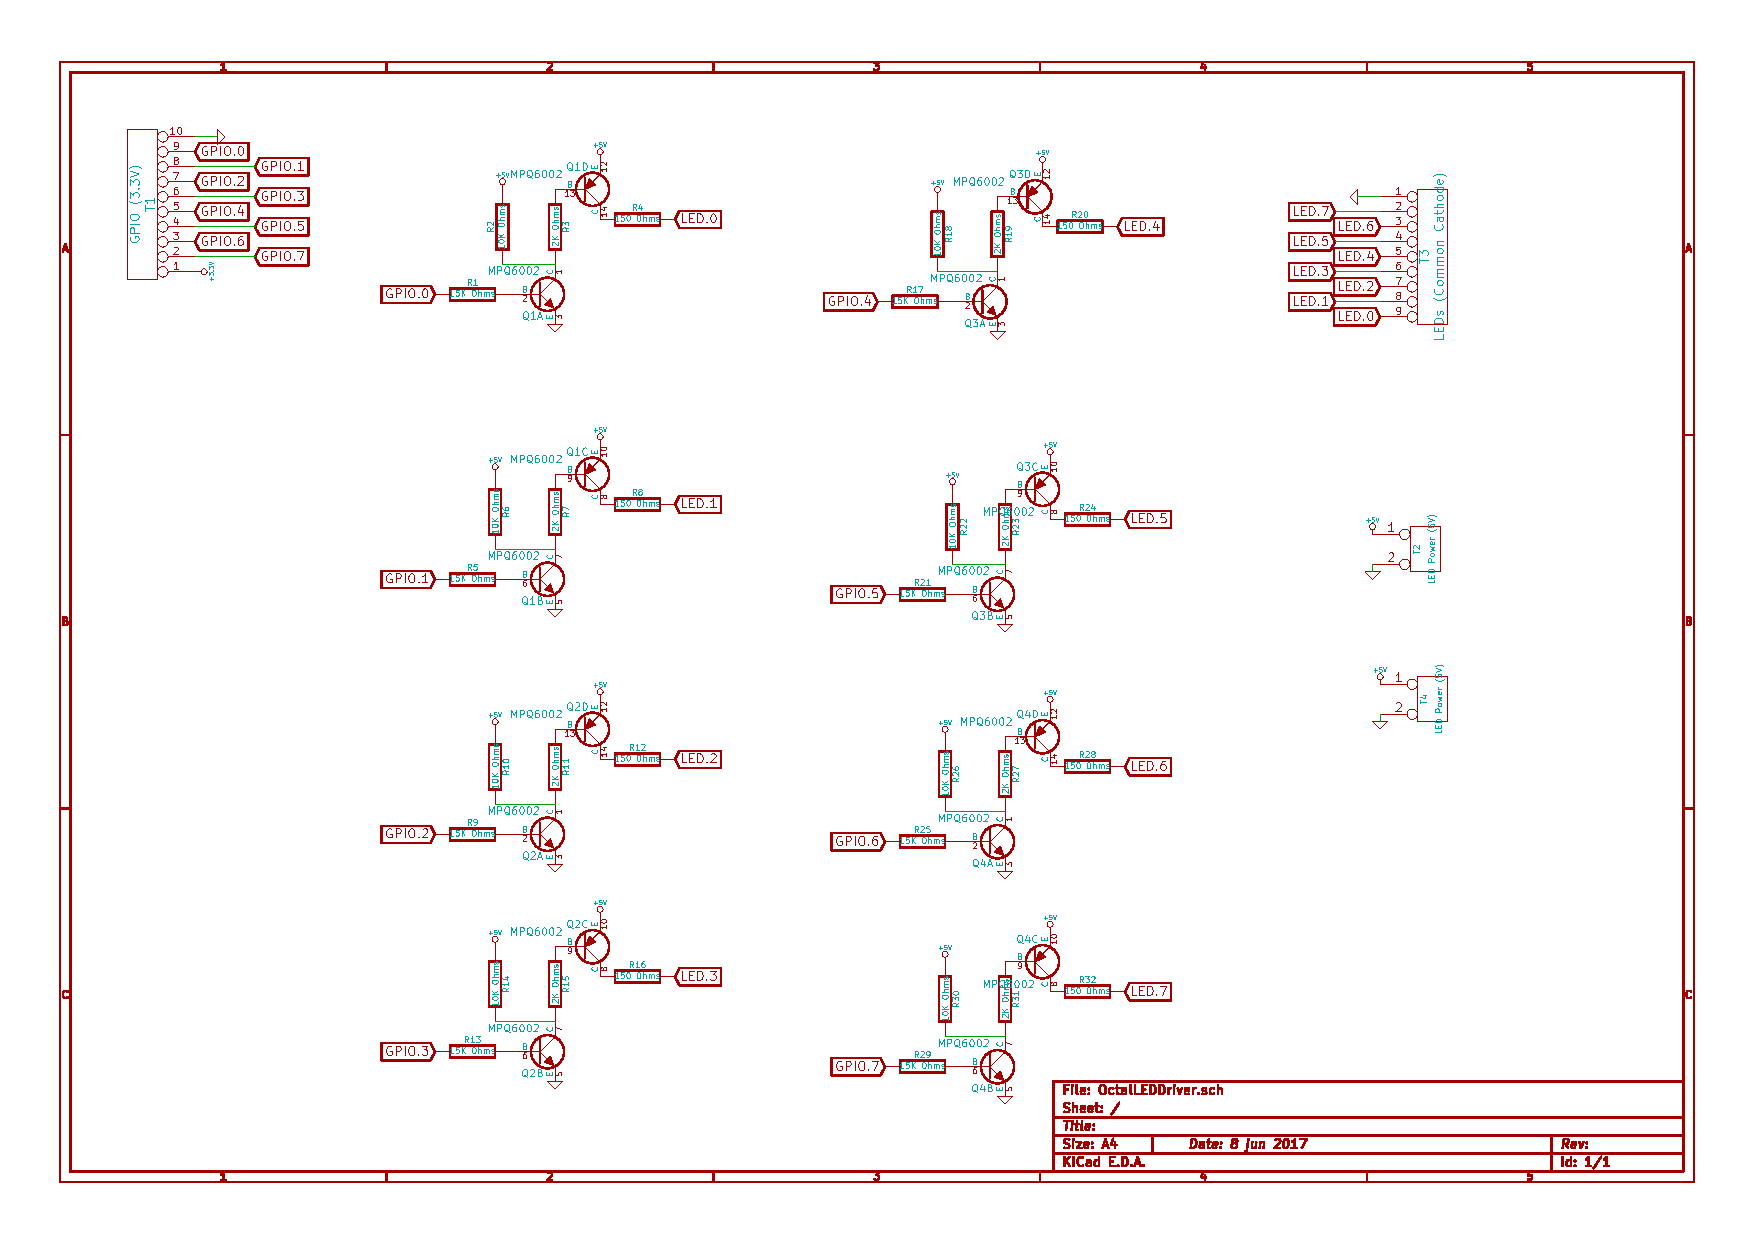
\includegraphics[width=5in]{OctalLEDDriver.pdf}
\caption{Circuit Diagram of the OctalLEDDriver}
\end{centering}\end{figure}
The circuit is just eight driver circuits, each featuring a NPN and a PNP
transistor, that level shift and buffer the 3V logic to 20 milliamp, 5V LED
drive circuits. The circuits include a current limiting series resistor, so
there is no need to include external resistors on your LEDs. The circuit
assumes 2V LEDs (typical of standard red, green, and yellow LEDs).

\section{Parts List}

\begin{table}[htp]
\begin{centering}\begin{tabular}{|l|l|p{1in}|l|}
\hline
Value&Quantity&References&Mouser Part Number\\
\hline
MPQ6002&4&Q1 Q2 Q3 Q4&610-MPQ6002\\
\hline
15K Ohms&8&R1 R5 R9 R13 R17 R21 R25 R29&603-CFR-25JR-5215K\\
\hline
10K Ohms&8&R2 R6 R10 R14 R18 R22 R26 R30&603-CFR-25JR-5210K\\
\hline
2K Ohms&8&R3 R7 R11 R15 R19 R23 R27 R31&603-CFR-25JR-522K\\
\hline
150 Ohms&8&R4 R8 R12 R16 R20 R24 R28 R32&588-OK1515E-R52\\
\hline
GPIO (3.3V)&1&T1&651-1725737 or 2x 651-1725685 \\
\hline
LED Power (5V)&2&T2 T4&651-1725656\\
\hline
LEDs (Common Cathode)&1&T3&651-1725724\\
\hline
\end{tabular}
\caption{Parts list for OctalLEDDriver boards.}
\end{centering}\end{table}\footnote{Mouser Project link: 
\url{http://www.mouser.com/ProjectManager/ProjectDetail.aspx?AccessID=f337ca3247}.}

The only parts that might be substituted are the screw terminal boards. Feel 
free to select either pin arrays or spring terminals for the terminals.

\section{Circuit Board Layout}

\begin{figure}[hbpt]\begin{centering}%
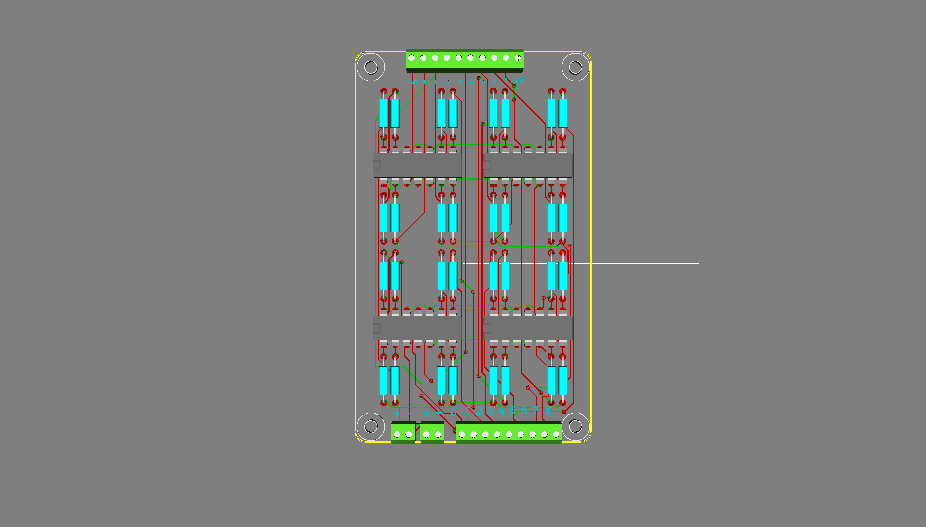
\includegraphics[width=5in]{OctalLEDDriver3DTop.png}
\caption{3D rendering of the OctalLEDDriver board}
\end{centering}\end{figure}
\begin{figure}[hbpt]\begin{centering}%
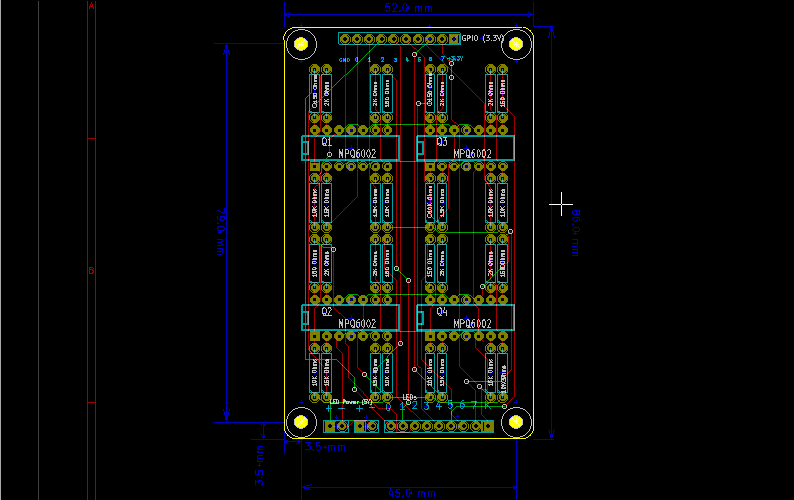
\includegraphics[width=5in]{OctalLEDDriver.png}
\caption{Fabrication image of the OctalLEDDriver board}
\end{centering}\end{figure}
Board assembly is straight forward. You need to be careful orienting the quad 
transistors. 

\section{Downloadables}

Full design information is available on GitHub here:
\url{https://github.com/RobertPHeller/RPi-RRCircuits/tree/master/OctalLEDDriver}.



